

This section elaborates the details of the design of \spl.
It cover the techniques / technology used and give detailed information about the layout of the parts.

The whole system is composed of modules, that communicate with each other.
\Figref{whole_setup} shows an overview of all the modules \spl consists of.

\begin{figure}[htbp]
  \centering
    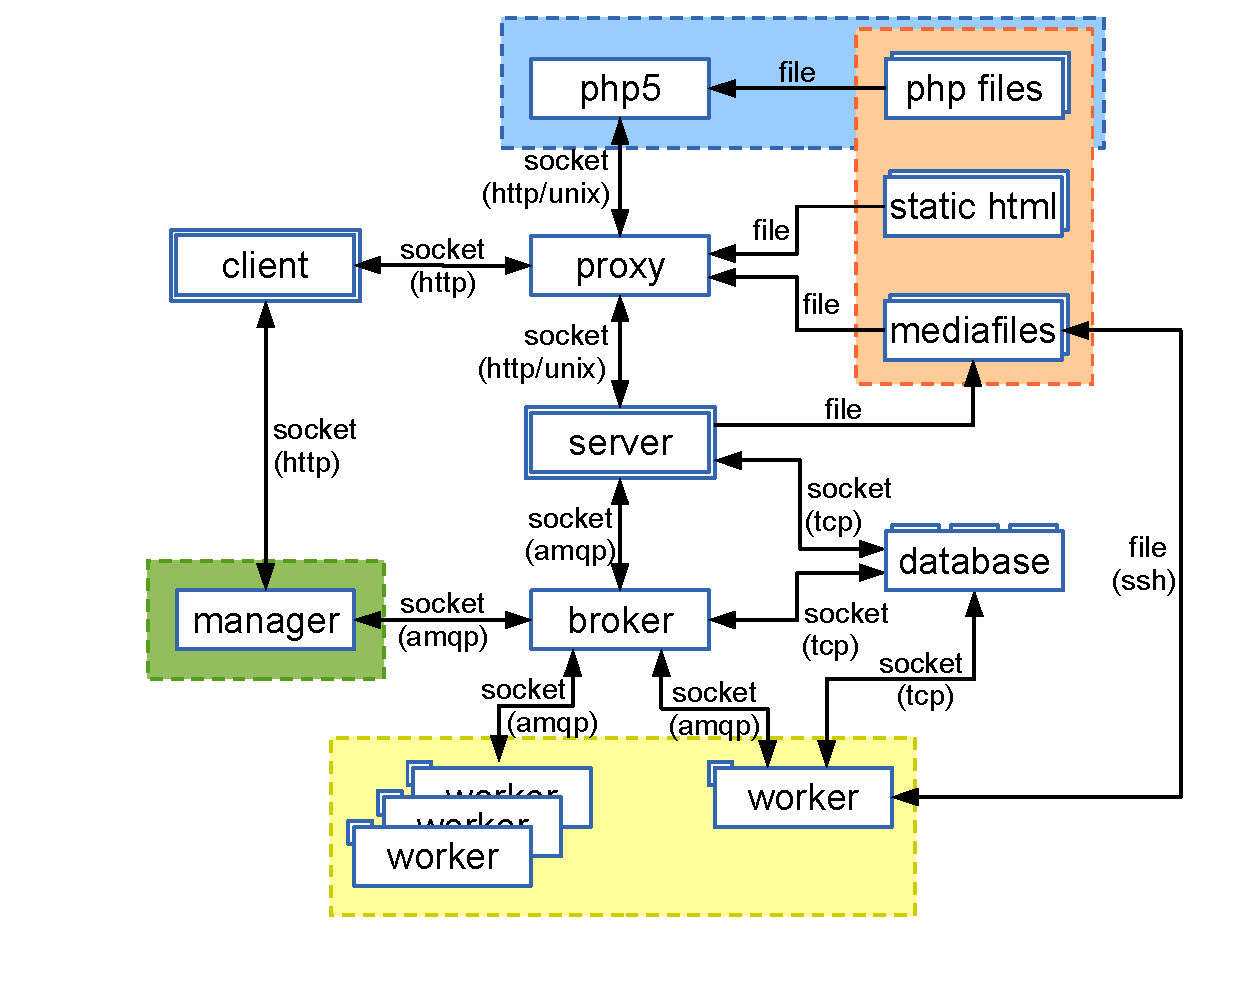
\includegraphics[width=\figwidth]{fig/whole_setup.pdf}
  \caption{\spl setup. The modules and their communicaion.}
  \label{fig:whole_setup}
\end{figure}

The setup shown here is the most extended setup.

The basic element needed for an webapp is a client side software (compare to a User Interface in traditional programming) and a server side software (compare to the business intelligence of an application.)


For other use cases like local installation, several parts can be removed.




